% Copyright 2004 by Till Tantau <tantau@users.sourceforge.net>.
%
% In principle, this file can be redistributed and/or modified under
% the terms of the GNU Public License, version 2.
%
% However, this file is supposed to be a template to be modified
% for your own needs. For this reason, if you use this file as a
% template and not specifically distribute it as part of a another
% package/program, I grant the extra permission to freely copy and
% modify this file as you see fit and even to delete this copyright
% notice. 

\documentclass{beamer}
% Replace the \documentclass declaration above
% with the following two lines to typeset your 
% lecture notes as a handout:
%\documentclass{article}
%\usepackage{beamerarticle}

\usepackage{graphicx}
\usepackage[utf8]{inputenc}
\usepackage{tabto}
 
\graphicspath{ {img/} }


% There are many different themes available for Beamer. A comprehensive
% list with examples is given here:
% http://deic.uab.es/~iblanes/beamer_gallery/index_by_theme.html
% You can uncomment the themes below if you would like to use a different
% one:
%\usetheme{AnnArbor}
%\usetheme{Antibes}
%\usetheme{Bergen}
%\usetheme{Berkeley}
%\usetheme{Berlin}
%\usetheme{Boadilla}
%\usetheme{boxes}
%\usetheme{CambridgeUS}
%\usetheme{Copenhagen}
%\usetheme{Darmstadt}
%\usetheme{default}
%\usetheme{Frankfurt}
%\usetheme{Goettingen}
%\usetheme{Hannover}
%\usetheme{Ilmenau}
%\usetheme{JuanLesPins}
%\usetheme{Luebeck}
%\usetheme{Madrid}
%\usetheme{Malmoe}
%\usetheme{Marburg}
%\usetheme{Montpellier}
%\usetheme{PaloAlto}
%\usetheme{Pittsburgh}
%\usetheme{Rochester}
%\usetheme{Singapore}
%\usetheme{Szeged}
\usetheme{Warsaw}

\title{Programming with Python}

% A subtitle is optional and this may be deleted
\subtitle{Lesson 4: Lists!}

%\author{F.~Author\inst{1} \and S.~Another\inst{2}}
% - Give the names in the same order as the appear in the paper.
% - Use the \inst{?} command only if the authors have different
%   affiliation.

%\institute[Universities of Somewhere and Elsewhere] % (optional, but mostly needed)
%{
%  \inst{1}%
%  Department of Computer Science\\
%  University of Somewhere
%  \and
%  \inst{2}%
%  Department of Theoretical Philosophy\\
%  University of Elsewhere}
% - Use the \inst command only if there are several affiliations.
% - Keep it simple, no one is interested in your street address.

\date{November 22th, 2016}
% - Either use conference name or its abbreviation.
% - Not really informative to the audience, more for people (including
%   yourself) who are reading the slides online

\subject{Python Lessons}
% This is only inserted into the PDF information catalog. Can be left
% out. 

% If you have a file called "university-logo-filename.xxx", where xxx
% is a graphic format that can be processed by latex or pdflatex,
% resp., then you can add a logo as follows:

% \pgfdeclareimage[height=0.5cm]{university-logo}{university-logo-filename}
% \logo{\pgfuseimage{university-logo}}

% Delete this, if you do not want the table of contents to pop up at
% the beginning of each subsection:
%\AtBeginSubsection[]
%{
%  \begin{frame}<beamer>{Outline}
%    \tableofcontents[currentsection,currentsubsection]
%  \end{frame}
%}

% Let's get started
\begin{document}

\begin{frame}
  \titlepage
\end{frame}

%\begin{frame}{Outline}
%  \tableofcontents
%  % You might wish to add the option [pausesections]
%\end{frame}

% Section and subsections will appear in the presentation overview
% and table of contents.
\section{Introduction \& Recap}

\begin{frame}{Last week's goals}
\pause
\begin{itemize}
  \item We have learnt about opening and closing files
  \pause
  \item We have learnt to write to, and read from files using the file object
  \pause
  \item We have learnt about the importance of functions and keeping code clean
  \pause
  \item We have used functions to make our code more readable, as well as to write to a log
\end{itemize}
  
\end{frame}

\section{Lists}

\begin{frame}{Goodbye calculator - you won't be missed}

Our calculator is finally complete!

\pause

Demonstration

\end{frame}

\begin{frame}{A recap on variables}

\begin{itemize}
  \item An integer (1,2,3 etc) \pause
  \item A character ('a','b','c' etc) \pause
  \item A string ("Hello, World!", "I love python xo" etc) \pause
  \item A float (1.45345, 24.4562389, 7.4234 etc) \pause
\end{itemize}

\end{frame}

\begin{frame}{One more type of variable - the list}
A list is a collection of variables.\\
\pause
It can be something like this:\\ \pause
{[}1, 1, 2, 3, 5, 8, 13{]}\\ \pause
It can be something like this:\\ \pause
{[}'h', 'e', 'l', 'l', 'o'{]}\\ \pause
It can even be something like this:\\ \pause
{[}"hello world", {[}1,5,7{]}, "my name is casper", 'a', "holy macaroni", 2.542{]}
\end{frame}

\begin{frame}{List operations}
To get an element from a list, you use square brackets:\\ \pause
\begin{figure}[h]
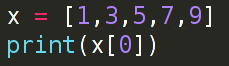
\includegraphics[width=0.7\textwidth]{squarebrack}
\end{figure}

\pause
This prints the value '1', as lists are zero-indexed (the list starts at element '0' and goes up from there).

\end{frame}


\begin{frame}{Printing out a list}

We can use a while loop to print each element in a list: \pause \\
\begin{figure}[h]
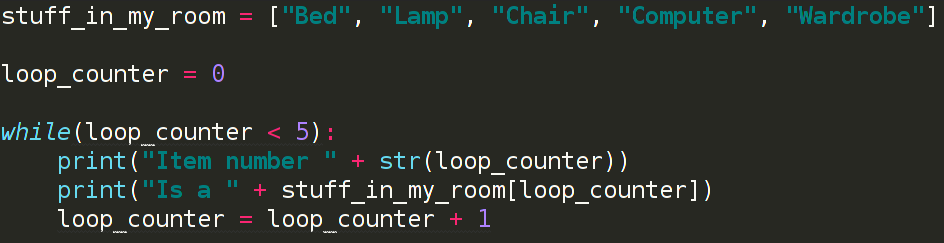
\includegraphics[width=0.9\textwidth]{roomstuff}
\end{figure}
\pause
However, the details are quite messy. We need to keep a loop counter variable and move it around.\\ \pause
We also have a fixed \textit{magic} number in the example, 5.

\end{frame}

\begin{frame}{The \textit{len()} function}

The \textit{len()} function takes in a list of something and returns the length of the list.\\ \pause
For example, \textit{len({[}1, 2, 4, 8, 16{]})} returns \textit{5} as there are 5 elements in {[}1, 2, 4, 8, 16{]}.\\ \pause
We can use this to remove the \textit{magic} number from our code.

\end{frame}

\begin{frame}{No more magic numbers}
\begin{figure}[h]
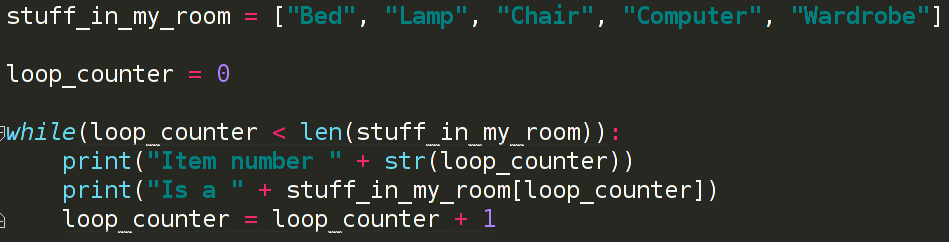
\includegraphics[width=0.9\textwidth]{roomstuff3}
\end{figure}
\pause
However, we still have to fiddle around with this \textit{loop counter}
\end{frame}

\begin{frame}{Introducing the for loop}

Along with the while loop, if we want to loop, we can use the for loop\\ \pause

Whereas the while loop would keep looping while a boolean was satisfied, the for loop instead does one \textit{loop} for each value in a list\\


\end{frame}

\begin{frame}{A for loop in action}

This is how the previous example looks like with a for loop:\\ \pause
\begin{figure}[h]
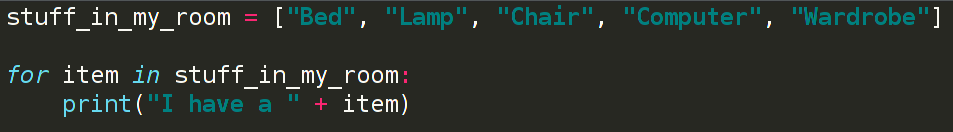
\includegraphics[width=0.9\textwidth]{roomstuff2}
\end{figure}

\end{frame}

\begin{frame}{Neat list functions}

Below are some neat list functions you may (or may not) need when using lists:
\pause

\begin{itemize}
  \item {[}1,2,3{]} + {[}4,5,7{]} \pause = {[}1,2,3,4,5,7{]} \pause
  \item {[}1,2,3{]} * 4 \pause = {[}1,2,3,1,2,3,1,2,3,1,2,3{]} \pause
  \item {[}1,2,3{]}.append(78) \pause = {[}1,2,3,78{]} \pause
  \item {[}1,2,3{]}.pop() \pause = {[}1,2{]} \pause
\end{itemize}

Note, if there's ever something you want to do which you are stuck on, google has tonnes of posts about pretty much everything to do with python.\\

\end{frame}

\section{Text-based Adventure}

\begin{frame}

With variables, loops, conditionals, file I/O and now lists we have a large and evergrowing toolkit of utensils we can use to produce high quality code.\\ \pause

It's now time to put it all into action!\\

\end{frame}

\begin{frame}

Live codin'\\
\pause
Now it's your go!
\end{frame}

\begin{frame}

\textbf{https://github.com/casper-oakley/python-lessons} \\

The skeleton I have just written can be found in the lesson4/src directory.\\ \pause

If you're looking for some ideas for cool things to add, why not try:
\begin{itemize}
  \item An inventory, based off a list
  \item A way to save and load your character from a file
  \item A really intricate storyline
\end{itemize}

\end{frame}

\section{Summary}

\begin{frame}{That's all for tonight}
  To summarise:
  \pause
  \begin{itemize}
  \item We learnt about lists\pause
  \item We learnt about how we can iterate on lists with a for loop\pause
  \item We learnt about some list operations\pause
  \item We begun writing our own text based game!
  \end{itemize}
\end{frame}

\begin{frame}{For next week}
Source code plus lecture slides will be available online soon after the lesson.\\
If you are new to HackSocNotts, please join us on \textit{http://hacksocnotts.slack.com}.\\
If you have any questions, feel free to ask now or over slack.\\
\end{frame}

\end{document}


